\chapter{Methods and testing}
\label{voidmeth}

So far we've only written short programs that have a single class and a single method (\java{main}).
In this chapter, we'll show you how to organize longer programs into multiple methods and classes.


%We will also take a look at separate compilation.
%At a conceptual level, a {\bf method} represents a mathematical {\em function} or a general {\em procedure}.
%Some methods perform a computation and return a result.
%For example, \java{Math.sqrt(25)} returns the value \java{5.0}.
%Other methods (including \java{main}) carry out a sequence of actions without returning a result.
%Java uses the keyword \java{void} to declare such methods.
%Regardless whether they return a value or not, methods enable you to break down a complex program into smaller blocks of code.


\section{Adding new methods}
\label{adding_methods}

\index{method!definition}

You have probably guessed by now that you can define more than one method in a class.
Here's an example:

\begin{trinket}[310]{NewLine.java}
public class NewLine {

    public static void newLine() {
        System.out.println();
    }

    public static void main(String[] args) {
        System.out.println("First line.");
        newLine();
        System.out.println("Second line.");
    }
}
\end{trinket}

\index{main}
\index{case-sensitive}

The name of the class is \java{NewLine}.
By convention, class names begin with a capital letter.
\java{NewLine} contains two methods, \java{newLine} and \java{main}.
Remember that Java is case-sensitive, so \java{NewLine} and \java{newLine} are not the same.

\index{camel case}

Method names should begin with a lowercase letter and use ``camel case'', which is a cute name for \java{jammingWordsTogetherLikeThis}.
You can use any name you want for methods, except \java{main} or any of the Java keywords.

\index{public}
\index{void}
\index{type!void}

\java{newLine} and \java{main} are \java{public}, which means they can be invoked from other classes.
They are both \java{static}, but we can't explain what that means yet.
And they are both \java{void}, which means that they don't yield a result (unlike the \java{Math} methods, for example).

\index{parameter}

The parentheses after the method name contain a list of variables, called {\bf parameters}, where the method stores its arguments.
\java{main} has a single parameter, called \java{args}, which has type \java{String[]}.
That means that whoever invokes \java{main} must provide an array of strings (we'll get to arrays in a later chapter).

Since \java{newLine} has no parameters, it requires no arguments, as shown when it is invoked in \java{main}.
And because \java{newLine} is in the same class as \java{main}, we don't have to specify the class name.

The output of this program is:

\begin{stdout}
First line.

Second line.
\end{stdout}

Notice the extra space between the lines.
If we wanted more space between them, we could invoke the same method repeatedly:

\begin{code}
public static void main(String[] args) {
    System.out.println("First line.");
    newLine();
    newLine();
    newLine();
    System.out.println("Second line.");
}
\end{code}

Or we could write a new method that displays three blank lines:

\begin{code}
public static void threeLine() {
    newLine();
    newLine();
    newLine();
}

public static void main(String[] args) {
    System.out.println("First line.");
    threeLine();
    System.out.println("Second line.");
}
\end{code}

You can invoke the same method more than once, and you can have one method invoke another.
In this example, \java{main} invokes \java{threeLine}, and \java{threeLine} invokes \java{newLine}.

Beginners often wonder why it is worth the trouble to create new methods.
There are many reasons, but this example demonstrates a few of them:

\begin{itemize}

\item Creating a new method gives you an opportunity to give a name to a group of statements, which makes code easier to read and understand.
%Methods simplify a program by hiding complex computations behind a single statement, and by using English words in place of arcane code.
%Which is clearer, \java{newLine} or \java{System.out.println()}?

\item Introducing new methods can make a program smaller by eliminating repetitive code.
For example, to display nine consecutive new lines, you could invoke \java{threeLine} three times.

\item A common problem solving technique is to break tasks down into sub-problems.
Methods allow you to focus on each sub-problem in isolation, and then compose them into a complete solution.

\end{itemize}

%Perhaps most importantly, organizing your code into multiple methods allows you to test individual parts of your program separately.
%It's easier to get a complex program working if you know that each sub-part works correctly.

%In Section~\ref{methods} we will come back to this question and list some additional benefits of dividing programs into methods.


\section{Flow of execution}

\index{class}
\index{method}

Pulling together the code from the previous section, the complete program looks like this:

\begin{trinket}{NewLine.java}
public class NewLine {

    public static void newLine() {
        System.out.println();
    }

    public static void threeLine() {
        newLine();
        newLine();
        newLine();
    }

    public static void main(String[] args) {
        System.out.println("First line.");
        threeLine();
        System.out.println("Second line.");
    }
}
\end{trinket}

\index{flow of execution}

When you look at a class definition that contains several methods, it is tempting to read it from top to bottom.
But that is likely to be confusing, because that is not the {\bf flow of execution} of the program.

Execution always begins at the first statement of \java{main}, regardless of where it is in the source file.
Statements are executed one at a time, in order, until you reach a method invocation, which you can think of as a detour.
Instead of going to the next statement, you jump to the first line of the invoked method, execute all the statements there, and then come back and pick up exactly where you left off.

That sounds simple enough, but remember that one method can invoke another one.
In the middle of \java{main}, we go off to execute the statements in \java{threeLine}.
While we are executing \java{threeLine}, we go off to execute \java{newLine}.
Then \java{newLine} invokes \java{println}, which causes yet another detour.

Fortunately, Java is good at keeping track of which methods are running.
So when \java{println} completes, it picks up where it left off in \java{newLine}; when \java{newLine} completes, it goes back to \java{threeLine}, and when \java{threeLine} completes, it gets back to \java{main}.

In summary, when you read a program, don't read from top to bottom.
Instead, follow the flow of execution.

%Technically, the program does not terminate at the end of \java{main}.
%Instead, execution picks up where it left off in the program that invoked \java{main}, which is the Java interpreter.
%The interpreter takes care of things like deleting windows and general cleanup, and {\em then} the program terminates.


\section{Parameters and arguments}

\index{parameter}
\index{argument}

Some of the methods we have used require arguments, which are the values you provide when you invoke the method.
For example, to find the sine of a number, you have to provide the number, so \java{sin} takes a \java{double} as an argument.
To display a message, you have to provide the message, so \java{println} takes a \java{String}.

When you use a method, you provide the arguments.
When you write a method, you name the parameters.
The parameter list indicates what arguments are required.
The following class shows an example:

\begin{trinket}[295]{PrintTwice.java}
public class PrintTwice {

    public static void printTwice(String s) {
        System.out.println(s);
        System.out.println(s);
    }

    public static void main(String[] args) {
        printTwice("Don't make me say this twice!");
    }
}
\end{trinket}

\java{printTwice} has a parameter named \java{s} with type \java{String}.
When we invoke \java{printTwice}, we have to provide an argument with type \java{String}.

Before the method executes, the argument gets assigned to the parameter.
In this example, the argument \java{"Don't make me say this twice!"} gets assigned to the parameter \java{s}.

\index{parameter passing}

This process is called {\bf parameter passing} because the value gets passed from outside the method to the inside.
An argument can be any kind of expression, so if you have a \java{String} variable, you can use it as an argument:

\begin{code}
String argument = "Never say never.";
printTwice(argument);
\end{code}

The value you provide as an argument must have the same type as the parameter.
For example, if you try:

\begin{code}
printTwice(17);  // syntax error
\end{code}

You will get an error message like this:

\begin{stdout}
File: Test.java  [line: 10]
Error: method printTwice in class Test cannot be applied
       to given types;
  required: java.lang.String
  found: int
  reason: actual argument int cannot be converted to
          java.lang.String by method invocation conversion
\end{stdout}

Sometimes Java can convert an argument from one type to another automatically.
For example, \java{Math.sqrt} requires a \java{double}, but if you invoke \java{Math.sqrt(25)}, the integer value \java{25} is automatically converted to the floating-point value \java{25.0}.
But in the case of \java{printTwice}, Java can't (or won't) convert the integer \java{17} to a \java{String}.

Parameters and other variables only exist inside their own methods.
Inside \java{main}, there is no such thing as \java{s}.
If you try to use it there, you'll get a compiler error.
Similarly, inside \java{printTwice} there is no such thing as \java{argument}.
That variable belongs to \java{main}.

\index{local variable}
\index{variable!local}

Because variables only exist inside the methods where they are defined, they are often called {\bf local variables}.


\section{Multiple parameters}
\label{time}

\index{parameter!multiple}
\index{method!parameters}

Here is an example of a method that takes two parameters:

\begin{code}
public static void printTime(int hour, int minute) {
    System.out.print(hour);
    System.out.print(":");
    System.out.println(minute);
}
\end{code}

In the parameter list, it may be tempting to write:

\begin{code}
public static void printTime(int hour, minute) {
    ...
\end{code}

But that format (without the second \java{int}) is only legal for variable declarations.
In parameter lists, you need to specify the type of each variable separately.

To invoke this method, we have to provide two integers as arguments:

\begin{code}
int hour = 11;
int minute = 59;
printTime(hour, minute);
\end{code}

A common error is to declare the types of the arguments, like this:

\begin{code}
int hour = 11;
int minute = 59;
printTime(int hour, int minute);  // syntax error
\end{code}

That's a syntax error; the compiler sees \java{int hour} and \java{int minute} as variable declarations, not expressions.
You wouldn't declare the types of the arguments if they were simply integers:

\begin{code}
printTime(int 11, int 59);  // syntax error
\end{code}


\section{Stack diagrams}
\label{stack}

Pulling together the code fragments from the previous section, here is a complete class definition:

\begin{trinket}[340]{PrintTime.java}
public class PrintTime {

    public static void printTime(int hour, int minute) {
        System.out.print(hour);
        System.out.print(":");
        System.out.println(minute);
    }

    public static void main(String[] args) {
        int hour = 11;
        int minute = 59;
        printTime(hour, minute);
    }
}
\end{trinket}

\java{printTime} has two parameters, named \java{hour} and \java{minute}.
And \java{main} has two variables, also named \java{hour} and \java{minute}.
Although they have the same names, these variables are not the same.
\java{hour} in \java{printTime} and \java{hour} in \java{main} refer to different storage locations, and they can have different values.

For example, you could invoke \java{printTime} like this:

\begin{code}
int hour = 11;
int minute = 59;
printTime(hour + 1, 0);
\end{code}

Before the method is invoked, Java evaluates the arguments; in this example, the results are \java{12} and \java{0}.
Then it assigns those values to the parameters.
Inside \java{printTime}, the value of \java{hour} is \java{12}, not \java{11}, and the value of \java{minute} is \java{0}, not \java{59}.
Furthermore, if \java{printTime} modifies one of its parameters, that change has no effect on the variables in \java{main}.

\index{stack diagram}
\index{diagram!stack}
\index{frame}

One way to keep track of everything is to draw a {\bf stack diagram}, which is a memory diagram (see Section~\ref{state}) that shows method invocations.
For each method there is a box called a {\bf frame} that contains the method's parameters and variables.
The name of the method appears outside the frame; the variables and parameters appear inside.

\begin{figure}[!ht]
\begin{center}
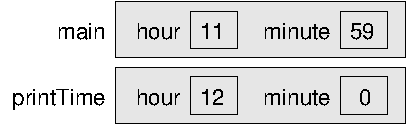
\includegraphics[scale=0.9]{figs/stack.pdf}
\caption{Stack diagram for \java{PrintTime}.}
\label{fig.stack}
\end{center}
\end{figure}

As with memory diagrams, stack diagrams show variables and methods at a particular point in time.
Figure~\ref{fig.stack} is a stack diagram at the beginning of the \java{printTime} method.

%\index{scope}

%Stack diagrams help you to visualize the {\bf scope} of a variable, which is the area of a program where a variable exists.


\section{Return values}

\index{void}

When you invoke a void method, the invocation is usually on a line all by itself.
For example, here is the \java{countup} method from Section~\ref{recursion}:

\begin{code}
public static void countup(int n) {
    if (n == 0) {
        System.out.println("Blastoff!");
    } else {
        countup(n - 1);
        System.out.println(n);
    }
}
\end{code}

And here is how it is invoked:

\begin{code}
countup(3);
System.out.println("Have a nice day.");
\end{code}

On the other hand, when you invoke a value method, you have to do something with the return value.
We usually assign it to a variable or use it as part of an expression, like this:

\begin{code}
double error = Math.abs(expected - actual);
double height = radius * Math.sin(angle);
\end{code}

\index{value method}
\index{method!value}

Compared to void methods, value methods differ in two ways:

\index{return type}
\index{return value}

\begin{itemize}

\item They declare the type of the return value (the {\bf return type});

\item They use at least one \java{return} statement to provide a {\bf return value}.

\end{itemize}

Here's an example: \java{calculateArea} takes a \java{double} as a parameter and returns the area of a circle with that radius:

\begin{code}
public static double calculateArea(double radius) {
    double result = Math.PI * radius * radius;
    return result;
}
\end{code}

As usual, this method is \java{public} and \java{static}.
But in the place where we are used to seeing \java{void}, we see \java{double}, which means that the return value from this method is a \java{double}.

\index{return}
\index{statement!return}

The last line is a new form of the \java{return} statement that includes a return value.
This statement means, ``return immediately from this method and use the following expression as the return value.''
The expression you provide can be arbitrarily complex, so we could have written this method more concisely:

\begin{code}
public static double calculateArea(double radius) {
    return Math.PI * radius * radius;
}
\end{code}

\index{temporary variable}
\index{variable!temporary}

On the other hand, {\bf temporary variables} like \java{result} often make debugging easier, especially when you are stepping through code using an interactive debugger (see Appendix~\ref{debugger}).

The type of the expression in the \java{return} statement must match the return type of the method.
When you declare that the return type is \java{double}, you are making a promise that this method will eventually produce a \java{double} value.
If you try to \java{return} with no expression, or an expression with the wrong type, the compiler will generate an error.

Sometimes it is useful to have multiple return statements, for example, one in each branch of a conditional:

\begin{code}
public static double absoluteValue(double x) {
    if (x < 0) {
        return -x;
    } else {
        return x;
    }
}
\end{code}

Since these \java{return} statements are in a conditional statement, only one will be executed.
As soon as either of them executes, the method terminates without executing any more statements.

\index{dead code}

Code that appears after a \java{return} statement (in the same block), or any place else where it can never be executed, is called {\bf dead code}.
The compiler will give you an ``unreachable statement'' error if part of your code is dead.
For example, this method contains dead code:

\begin{code}
public static double absoluteValue(double x) {
    if (x < 0) {
        return -x;
    } else {
        return x;
    }
    System.out.println("This line is dead.");
}
\end{code}

If you put \java{return} statements inside a conditional statement, you have to make sure that {\em every possible path} through the program reaches a \java{return} statement.
The compiler will let you know if that's not the case.
For example, the following method is incomplete:

\begin{code}
public static double absoluteValue(double x) {
    if (x < 0) {
        return -x;
    } else if (x > 0) {
        return x;
    }
    // syntax error
}
\end{code}

When \java{x} is 0, neither condition is true, so the method ends without hitting a return statement.
The error message in this case might be something like ``missing return statement'', which is confusing since there are already two of them.
But hopefully you will know what it means.


\section{Writing methods}
\label{distance}

\index{incremental development}
\index{program development}

Beginners often make the mistake of writing a lot of code before they try to compile and run it.
Then they spend way too much time debugging.
A better approach is what we call {\bf incremental development}.
The key aspects of incremental development are:

\begin{itemize}

\item Start with a working program and make small, incremental changes.
At any point, if there is an error, you will know where to look.

\item Use variables to hold intermediate values so you can check them, either with print statements or by using a debugger.

\item Once the program is working, you can consolidate multiple statements into compound expressions (but only if it does not make the program more difficult to read).

\end{itemize}

As an example, suppose you want to find the distance between two points, given by the coordinates $(x_1, y_1)$ and $(x_2, y_2)$.
By the usual definition:

\[ distance = \sqrt{(x_2 - x_1)^2 +(y_2 - y_1)^2} \]

The first step is to consider what a \java{distance} method should look like in Java.
In other words, what are the inputs (parameters) and what is the output (return value)?
In this case, the two points are the parameters, and it is natural to represent them using four \java{double} values.
%, although we will see later that there is a \java{Point} object in Java that we could use.
The return value is the distance, which should also have type \java{double}.

\index{stub}

Already we can write an outline for the method, which is sometimes called a {\bf stub}.
The stub includes the method signature and a \java{return} statement:

\begin{code}
public static double distance
        (double x1, double y1, double x2, double y2) {
    return 0.0;
}
\end{code}

The return statement is a placeholder that is necessary for the program to compile.
At this stage the program doesn't do anything useful, but it is good to compile it so we can find any syntax errors before we add more code.

It's usually a good idea to think about testing {\em before} you develop new methods; doing so can help you figure out how to implement them.
To test the method, we can invoke it from \java{main} using sample values:

\begin{code}
double dist = distance(1.0, 2.0, 4.0, 6.0);
\end{code}

With these values, the horizontal distance is 3.0 and the vertical distance is 4.0.
So the result should be 5.0, the hypotenuse of a 3-4-5 triangle.
When you are testing a method, it is helpful to know the right answer.

Once we have compiled the stub, we can start adding lines of code one at a time.
After each incremental change, we recompile and run the program.
If there is an error at any point, we have a good idea where to look: the last line we added.

The next step is to find the differences $x_2 - x_1$ and $y_2 - y_1$.
We store those values in temporary variables named \java{dx} and \java{dy}.

\begin{code}
public static double distance
        (double x1, double y1, double x2, double y2) {
    double dx = x2 - x1;
    double dy = y2 - y1;
    System.out.println("dx is " + dx);
    System.out.println("dy is " + dy);
    return 0.0;
}
\end{code}

\index{scaffolding}

The print statements allows us to check the intermediate values before proceeding.
They should be 3.0 and 4.0.
We will remove the print statements when the method is finished.
Code like that is called {\bf scaffolding}, because it is helpful for building the program, but it is not part of the final product.

The next step is to square \java{dx} and \java{dy}.
We could use the \java{Math.pow} method, but it is simpler to multiply each term by itself.

\begin{code}
public static double distance
        (double x1, double y1, double x2, double y2) {
    double dx = x2 - x1;
    double dy = y2 - y1;
    double dsquared = dx * dx + dy * dy;
    System.out.println("dsquared is " + dsquared);
    return 0.0;
}
\end{code}

Again, you should compile and run the program at this stage and check the intermediate value, which should be 25.0.
Finally, we can use \java{Math.sqrt} to compute and return the result.

\begin{code}
public static double distance
        (double x1, double y1, double x2, double y2) {
    double dx = x2 - x1;
    double dy = y2 - y1;
    double dsquared = dx * dx + dy * dy;
    double result = Math.sqrt(dsquared);
    return result;
}
\end{code}

%In \java{main}, we can print and check the value of the result.

As you gain more experience programming, you might write and debug more than one line at a time.
Nevertheless, incremental development can save you a lot of time.


\section{Method composition}

\index{composition}

Once you define a new method, you can use it as part of an expression, or build new methods using existing methods.
For example, suppose someone gave you two points, the center of the circle and a point on the perimeter, and asked for the area of the circle.
Let's say the center point is stored in the variables \java{xc} and \java{yc}, and the perimeter point is in \java{xp} and \java{yp}.

The first step is to find the radius of the circle, which is the distance between the two points.
Fortunately, we have a method that does just that (\java{distance}).

\begin{code}
double radius = distance(xc, yc, xp, yp);
\end{code}

The second step is to find the area of a circle with that radius.
We have a method for that computation too (\java{calculateArea}).

\begin{code}
double area = calculateArea(radius);
return area;
\end{code}

Putting everything together in a new method, we get:

\begin{code}
public static double circleArea
        (double xc, double yc, double xp, double yp) {
    double radius = distance(xc, yc, xp, yp);
    double area = calculateArea(radius);
    return area;
}
\end{code}

The temporary variables \java{radius} and \java{area} are useful for development and debugging, but once the program is working we can make it more concise by composing the method calls:

\begin{code}
public static double circleArea
        (double xc, double yc, double xp, double yp) {
    return calculateArea(distance(xc, yc, xp, yp));
}
\end{code}

\index{functional decomposition}

This example demonstrates a process called {\bf functional decomposition}; that is, breaking a complex computation into simple methods, testing the methods in isolation, and then composing the methods to perform the computation.
This process reduces debugging time and yields code that is more likely to be correct and easier to maintain.

%Computer scientists deal with the complexity of large programs by breaking down computations into simple methods (which in turn may call other methods).
%Data is passed around the program via method parameters and return statements.
%By using incremental development, scaffolding, and testing, you can be confident that your code is correct.


\section{Overloading}
\label{overloading}

You might have noticed that \java{circleArea} and \java{calculateArea} perform similar functions.
They both find the area of a circle, but they take different parameters.
For \java{calculateArea}, we have to provide the radius; for \java{circleArea} we provide two points.

\index{overload}

If two methods do the same thing, it is natural to give them the same name.
Having more than one method with the same name is called {\bf overloading}, and it is legal in Java as long as each version takes different parameters.
So we could rename \java{circleArea} to \java{calculateArea}:

\begin{code}
public static double calculateArea
        (double xc, double yc, double xp, double yp) {
    return calculateArea(distance(xc, yc, xp, yp));
}
\end{code}

Note that this new \java{calculateArea} method is {\em not} recursive.
When you invoke an overloaded method, Java knows which version you want by looking at the arguments that you provide.
If you write:

\begin{code}
double x = calculateArea(3.0);
\end{code}

Java looks for a method named \java{calculateArea} that takes one \java{double} as an argument, and so it uses the first version, which interprets the argument as a radius.
If you write:

\begin{code}
double y = calculateArea(1.0, 2.0, 4.0, 6.0);
\end{code}

Java uses the second version of \java{calculateArea}, which interprets the arguments as two points.
In this example, the second version actually invokes the first version.

Many Java methods are overloaded, meaning that there are different versions that accept different numbers or types of parameters.
For example, there are versions of \java{print} and \java{println} that accept a single parameter of any data type.
In the \java{Math} class, there is a version of \java{abs} that works on \java{double}s, and there is also a version for \java{int}s.

Although overloading is a useful feature, it should be used with caution.
You might get yourself nicely confused if you are trying to debug one version of a method while accidentally invoking a different one.


\section{Boolean methods}
\label{boolean}

\index{boolean}
\index{method!boolean}

Methods can return \java{boolean} values, just like any other type, which is often convenient for hiding tests inside methods.
For example:

\begin{code}
public static boolean isSingleDigit(int x) {
    if (x > -10 && x < 10) {
        return true;
    } else {
        return false;
    }
}
\end{code}

The name of this method is \java{isSingleDigit}.
It is common to give \java{boolean} methods names that sound like yes/no questions.
Since the return type is \java{boolean}, the return statement has to provide a boolean expression.

The code itself is straightforward, although it is longer than it needs to be.
Remember that the expression \java{x > -10 && x < 10} has type \java{boolean}, so there is nothing wrong with returning it directly (without the \java{if} statement):

\begin{code}
public static boolean isSingleDigit(int x) {
    return x > -10 && x < 10;
}
\end{code}

In \java{main}, you can invoke the method in the usual ways:

\begin{code}
System.out.println(isSingleDigit(2));
boolean bigFlag = !isSingleDigit(17);
\end{code}

The first line displays \java{true} because 2 is a single-digit number.
The second line sets \java{bigFlag} to \java{true}, because 17 is {\em not} a single-digit number.

Conditional statements often invoke \java{boolean} methods and use the result as the condition:

\begin{code}
if (isSingleDigit(z)) {
    System.out.println("z is small");
} else {
    System.out.println("z is big");
}
\end{code}

Examples like this one almost read like English:
``If is single digit z, print ... else print ...''.


\section{Vocabulary}

\begin{description}

% Note: expanded definition from Chapter 1
%\term{method}
%A named sequence of statements that performs a procedure or function.
%Methods may or may not take parameters, and may or may not return a value.

\term{invoke}
To cause a method to execute.
Also known as ``calling'' a method.

\term{parameter}
A piece of information that a method requires before it can run.
Parameters are variables: they contain values and have types.

% Note: expanded definition from Chapter 2
%\term{composition}
%The ability to combine simple expressions and statements into compound %expressions and statements, making it possible to use intermediate %computations as arguments.

\term{flow of execution}
The order in which Java executes methods and statements.
It may not necessarily be from top to bottom, left to right.

\term{parameter passing}
The process of assigning an argument value to a parameter variable.

\term{local variable}
A variable declared inside a method.
Local variables cannot be accessed from outside their method.

\term{stack diagram}
A graphical representation of the variables belonging to each method.
The method calls are ``stacked'' from top to bottom, in the flow of execution.

\term{frame}
In a stack diagram, a representation of the variables and parameters for a method, along with their current values.

%\term{scope}
%The area of a program where a variable exists.

\term{signature}
The first line of a method that defines its name, return type, and parameters.

\term{Javadoc}
A tool that reads Java source code and generates documentation in HTML format.

\term{documentation}
Comments that describe the technical operation of a class or method.

\end{description}


\section{Exercises}

The code for this chapter is in the {\tt ch05} directory of {\tt ThinkJava2Code}.
See page~\pageref{code} for instructions on how to download the repository.
Before you start the exercises, we recommend that you compile and run the examples.

If you have not already read Appendix~\ref{debugger}, now might be a good time.
It describes the DrJava debugger, which is a useful tool for tracing the flow of execution.


\begin{exercise}

The point of this exercise is to practice reading code and to make sure that you understand the flow of execution through a program with multiple methods.

\begin{enumerate}

\item What is the output of the following program?
Be precise about where there are spaces and where there are newlines.

{\it Hint:} Start by describing in words what \java{ping} and \java{baffle} do when they are invoked.

\item Draw a stack diagram that shows the state of the program the first time \java{ping} is invoked.

\item What happens if you invoke \java{baffle();} at the end of the \java{ping} method? (We will see why in the next chapter.)

\end{enumerate}

\begin{code}
public static void zoop() {
    baffle();
    System.out.print("You wugga ");
    baffle();
}

public static void main(String[] args) {
    System.out.print("No, I ");
    zoop();
    System.out.print("I ");
    baffle();
}

public static void baffle() {
    System.out.print("wug");
    ping();
}

public static void ping() {
    System.out.println(".");
}
\end{code}

\end{exercise}


%\begin{exercise}

%What is the difference between a variable and a method?
%In terms of their syntax, how does the Java compiler tell the difference between the two?

%%A variable is a {\em location of data}, whereas a method is a {\em location of code}.
%%In Java, methods always have parentheses, even if they have no arguments like \java{System.out.println()}.

%\end{exercise}


%ABD: We don't need this anymore since we used this as an example
%\begin{exercise}
%Draw a stack diagram that shows the state of the program in Section~\ref{time} when \java{main} invokes \java{printTime} with the arguments \java{11} and \java{59}.
%\end{exercise}


\begin{exercise}

The point of this exercise is to make sure you understand how to write and invoke methods that take parameters.

\begin{enumerate}
\item Write the first line of a method named \java{zool} that takes three parameters: an \java{int} and two \java{String}s.

\item Write a line of code that calls \java{zool}, passing as arguments the value \java{11}, the name of your first pet, and the name of the street you grew up on.
\end{enumerate}

\end{exercise}


\begin{exercise}

The purpose of this exercise is to take code from a previous exercise and encapsulate it in a method that takes parameters.
You should start with a working solution to Exercise~\ref{ex:date}.

\begin{enumerate}

\item Write a method called \java{printAmerican} that takes the day, date, month and year as parameters and that displays them in American format.

\item Test your method by invoking it from \java{main} and passing appropriate arguments.
The output should look something like this (except that the date might be different):

\begin{stdout}
Saturday, July 22, 2015
\end{stdout}

\item Once you have debugged \java{printAmerican}, write another method called \java{printEuropean} that displays the date in European format.

\end{enumerate}

\end{exercise}


\begin{exercise}
For the following program:

\begin{enumerate}

\item Draw a stack diagram that shows the state of the program the {\it second} time \java{zoop} is invoked.

\item What is the complete output?

\end{enumerate}

\begin{code}
public static void zoop(String fred, int bob) {
    System.out.println(fred);
    if (bob == 5) {
        ping("not ");
    } else {
        System.out.println("!");
    }
}

public static void main(String[] args) {
    int bizz = 5;
    int buzz = 2;
    zoop("just for", bizz);
    clink(2 * buzz);
}
\end{code}

\begin{code}
public static void clink(int fork) {
    System.out.print("It's ");
    zoop("breakfast ", fork);
}

public static void ping(String strangStrung) {
    System.out.println("any " + strangStrung + "more ");
}
\end{code}
\end{exercise}


\begin{exercise}

Draw a stack diagram that shows the state of the program in Section~\ref{recursion} after \java{main} invokes \java{nLines} with the parameter \java{n == 4}, just before the last invocation of \java{nLines} returns.

\end{exercise}


\begin{exercise}

Fermat's Last Theorem says that there are no integers $a$, $b$, and $c$ such that $a^n + b^n = c^n$, except when $n \leq 2$.

Write a method named \java{checkFermat} that takes four integers as parameters -- \java{a}, \java{b}, \java{c} and \java{n} -- and checks to see if Fermat's theorem holds.
If $n$ is greater than 2 and $a^n + b^n = c^n$, the program should display ``Holy smokes, Fermat was wrong!''
Otherwise the program should display ``No, that doesn't work.''

{\it Hint:} You may want to use \java{Math.pow}.

\end{exercise}


\begin{exercise}

The purpose of this exercise is to take a problem and break it into smaller problems, and to solve the smaller problems by writing simple methods.
Consider the first verse of the song ``99 Bottles of Beer'':

\begin{quote}
99 bottles of beer on the wall,\\
99 bottles of beer,\\
ya' take one down, ya' pass it around,\\
98 bottles of beer on the wall.
\end{quote}

Subsequent verses are identical except that the number of bottles gets smaller by one in each verse, until the last verse:

\begin{quote}
No bottles of beer on the wall,\\
no bottles of beer,\\
ya' can't take one down, ya' can't pass it around,\\
'cause there are no more bottles of beer on the wall!
\end{quote}

And then the song (finally) ends.

Write a program that displays the entire lyrics of ``99 Bottles of Beer''.
Your program should include a recursive method that does the hard part, but you might want to write additional methods to separate other parts of the program.
As you develop your code, test it with a small number of verses, like \java{3}.

\end{exercise}


\begin{exercise}

This exercise reviews the flow of execution through a program with multiple methods.
Read the following code and answer the questions.

\begin{code}
public class Buzz {

    public static void baffle(String blimp) {
        System.out.println(blimp);
        zippo("ping", -5);
    }

    public static void zippo(String quince, int flag) {
        if (flag < 0) {
            System.out.println(quince + " zoop");
        } else {
            System.out.println("ik");
            baffle(quince);
            System.out.println("boo-wa-ha-ha");
        }
    }

    public static void main(String[] args) {
        zippo("rattle", 13);
    }

}
\end{code}

\begin{enumerate}

\item Write the number {\tt 1} next to the first line of code in this program that will execute.

\item Write the number {\tt 2} next to the second line of code, and so on until the end of the program.
If a line is executed more than once, it might end up with more than one number next to it.

\item What is the value of the parameter \java{blimp} when \java{baffle} gets invoked?

\item What is the output of this program?

\end{enumerate}

\end{exercise}
